\section{Background}

This section contains basic knowledge that is necessary for the understanding of the rest of the thesis.
It briefly touches on artificial neural networks and convolutional neural networks in the beginning.
The subsection after that goes on to describe autoencoders in general. Next up, Kullback-Leibler divergence
is explained in detail as it is an essential part for the variational autoencoders as they are used in this
work. The difference between those variational autoencoders and the standard autoencoder is covered in the 
next subsection. At last, the dimensionality reduction methods principal component analysis and 
t-distributed stochastic neighbor embedding is brought up since they are used in this work to gain an 
understanding of the high dimensional latent space of the autoencoders.

\subsection{Remote Sensing Imagery}



\subsection{Artificial Neuron}

Inspired by biological neurons an artificial neuron has one or more weighted inputs that are summed together
and after that passed through a non-linear function called activation function. The output models the axon
of a biological neuron to which other biological neurons can connect via their dendrites which is similar
to an artificial neuron using the output of another artificial neuron as its input. 
By adjusting the separate weights of the inputs a single neuron is able to model
simple functions like the logic $and$ or the logic $or$.

\begin{figure}[h]
    \centering
    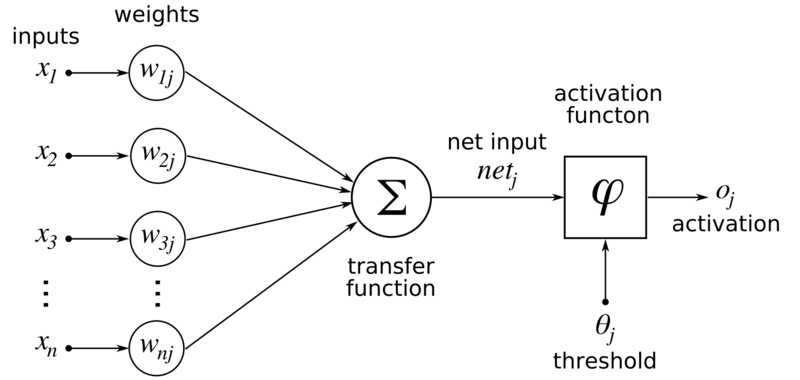
\includegraphics[width=0.7\textwidth]{images/figures/artificial_neuronHOML.png}
    \caption{An artificial neuron. Image taken from \parencite{1005-chrislb-artificial-neuron}}
\end{figure}


\subsection{Artificial Neural Network}



\subsection{Convolutional Neural Networks}



\subsection{Autoencoders}



\subsection{Kullback-Leibler Divergence}

\subsubsection{Entropy}

A part of the loss function used in the variational autoencoder is based on Kullback-Leibler divergence.
To understand Kullback-Leibler divergence it seems necessary to explain entropy from
the field of information theory. In short, entropy is a measure for the minimum average size an
encoding for a piece of information can possibly have.

Suppose there is a system $S1$ that can have four different states $a, b, c, d$
and every one of those states is equally likely to occur, that means the probability $P(x)$
of each state $x$ is $1/4$. Now the goal is to losslessly transmit all information about that system
with the minimum average amount of bits. That can be done with only two bits for example like this

\begin{center}
    \begin{tabular} {c c c c}
        $a: 00$ & $b: 01$ & $c: 10$ & $d: 11$
    \end{tabular}
\end{center}

However, if $P(a)=1$ and $P(b)=P(c)=P(d)=0,$ zero bits will suffice to encode the information since
it is always certain that the system is in state a. So the entropy of the system clearly depends on
the probabilities of each state. To see in which way, one can consider the system $S2$ with 
$P(a)=1/2,\ P(b)=1/4,\ P(c)=1/8$ and $P(d)=1/8$. In that case it would be best to encode the state
with the highest probability with as few bits as possible since it has to be transmitted the most
often. That means $a$ is encoded with one bit as $0$. When decoding the information there must be
no ambiguities so while the encoding for $b$ has to start with a $1$ it cannot be $1$ since we need 
to encode two more states so $b: 10$. Additionally if $c: 11$ there would be no space left for $d$:
say $d: 111$ then if the transmitted information is $111111\dots$ it could either be decoded to
$ccc\dots$ or $dd\dots$. So $c$ should rather be encoded as $110$ which way $d: 111$ works. In the end a valid
encoding that can transmit all information with the minimum average amount of bits is

\begin{center}
    \begin{tabular} {c c c c}
        $a: 0$ & $b: 10$ & $c: 110$ & $d: 111$
    \end{tabular}
\end{center}

Here the states $c, d$ are encoded with three bits instead of the two bits in the first example.
But $c$ and $d$ are transmitted far less often than $a$ which now only needs one bit. To be more precise
half of all transmissions have one bit. Additionally a quarter of all transmissions have two bits. 
The sum of those probabilities multiplied with the respective amount of bits is the average amount of bits
needed to transfer the information in a given encoding. So in the example, with $f(x)$ as the number of
bits that encode a state $x$, that turns out to be $P(a)f(a)+P(b)f(b)+P(c)f(c)+P(d)f(d)=1.75$.
That means for $S2$ on average you only need $1.75$ bits to encode a state and since that is also the
minimum $1.75$ is the entropy of $S2$.

In general in an optimal encoding $f(x)$ is the same as $\log_{2} \frac{1}{P(x)}$. For $S1$ $P(x)$ is $1/4$
so the number of bits for $x$ is $\log_{2} (4)=2$ what matches the two bits the first encoding uses 
for the states of $S1$.

The entropy $H$ of a system with a set of discrete events $X$ and the probability distribution $P(x)$
for each $x\in X$ is
\begin{equation}
    H(P)=\sum_{x\in X} P(x)\log_{2} \frac{1}{P(x)} = -\sum_{x\in X} P(x)\log_{2} P(x)
\end{equation}
This is often written as the expectation for a  given state $x$ under the distribution $P$.
\[ H(P)=E_{x\sim P}[-log_{2}P(x)]\]
Intuitively if a system has high entropy, the size of the encodings are high on average and many states
have small probabilities. This means it is hard to predict what state the system will be in at a given time
since there is no state that can be guessed with high confidence. If entropy is low, zero for example,
one can be confident that the system is in a certain state like in the previous example with $P(a)=1$.

%wie muss hier der fall P(x) = 0 abgesichert werden weil log(0) und 1/0 ?

\subsubsection{Cross Entropy}

If the real distribution $P$ of a system is unknown an estimate distribution $Q$ could be guessed
and encoding sizes $-log_{2}Q(x)$ can be produced which will not be optimal for the true distribution
$P$. Now with some data gathered and $P$ known the used encoding sizes can be cross-checked with the
expectation under the actual distribution resulting in the cross entropy $H(P,Q)$
\begin{equation}
    H(P,Q)=E_{x\sim P}[-log_{2}Q(x)]=-\sum_{x\in X} P(x)\log_{2} (Q(x))
\end{equation}
In machine learning tasks regarding classification this is often used as a loss function since the
label of a piece of data gives us a distribution $P$ with absolute certainty and $H(P)=0$. With the
inaccurate distribution $Q$ that the model estimates $H(P,Q)$ will be greater than zero unless
$P=Q$ where $H(P,Q)=H(P,P)=H(P)=0$. So the learning algorithm can try to minimize $H(P,Q)$.

\subsubsection{Kullback-Leibler Divergence}

Having computed the entropy $H(P)$ and cross-entropy $H(P,Q)$ of two distributions $P,\ Q$ it is 
possible to compare those distributions by comparing $H(P)$ and $H(P,Q)$ through subtraction
\begin{equation} \label{eq1}
    \begin{split}
        D_{KL}(P\parallel Q)    & = H(P,Q)-H(P) \\
                                & = E_{x\sim P}[-log_{2}Q(x)]-E_{x\sim P}[-log_{2}P(x)]\\
                                & = E_{x\sim P}[-log_{2}Q(x)+log_{2}P(x)]\\
                                & = E_{x\sim P}[log_{2}\frac{P(x)}{Q(x)}]\\
                                & = \sum_{x\in X} P(x)log_{2}\frac{P(x)}{Q(x)}
    \end{split}
\end{equation}
where $D_{KL}(P\parallel Q)$ is called the Kullback-Leibler divergence of $P$ and $Q$. This works
because $D_{KL}(P\parallel Q)$ is zero if $Q$ and $P$ are the same since that means $H(P,Q)=H(P)$.
On the opposite if $Q$ is different from $P$ then $H(P,Q)$ is greater than $H(P)$ and therefore 
the KL divergence is greater than zero proportional to how different $Q$ and $P$ are.
In summary Kullback-Leibler divergence is a measure of how different two probability distributions
are that is zero if they are the same and greater than zero if not.

\subsection{Variational Autoencoders}



\subsection{Principal Component Analysis}



\subsection{t-Distributed Stochastic Neighbor Embedding}